\documentclass[border=4pt]{standalone}
\usepackage{amsmath,amssymb,pgfplots}\pgfplotsset{compat=1.18}
\definecolor{figB}{RGB}{31,90,166}\definecolor{figR}{RGB}{176,48,48}\definecolor{figG}{RGB}{46,125,50}\definecolor{figO}{RGB}{214,120,20}
\begin{document}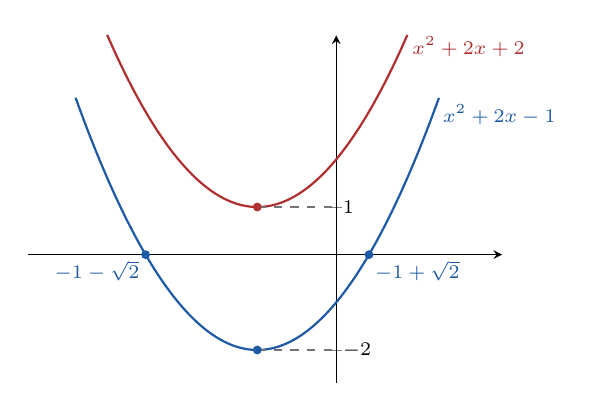
\begin{tikzpicture}
\begin{axis}[width=7.6cm,height=6cm,axis lines=middle,axis line style={-stealth,thin},
  xmin=-3.9,xmax=2.1,ymin=-2.7,ymax=4.6,xtick=\empty,ytick={-2,1},y tick label style={anchor=west,xshift=1pt},
  ticklabel style={font=\scriptsize},samples=120,domain=-3.3:1.3,clip=false]
\addplot[figR,thick,domain=-2.9:0.9] {x^2+2*x+2} node[pos=0.97,right,font=\scriptsize]{$x^2+2x+2$};
\addplot[figB,thick] {x^2+2*x-1} node[pos=0.97,right,font=\scriptsize]{$x^2+2x-1$};
% vertices at x = -b/2 = -1
\draw[dashed,black!55] (axis cs:-1,1)--(axis cs:0,1); \draw[dashed,black!55] (axis cs:-1,-2)--(axis cs:0,-2);
\fill[figR] (axis cs:-1,1) circle (1.6pt);
\fill[figB] (axis cs:-1,-2) circle (1.6pt);
% real zeros of the second one: -1 +- sqrt 2
\fill[figB] (axis cs:-2.4142,0) circle (1.6pt); \fill[figB] (axis cs:0.4142,0) circle (1.6pt);
\node[figB,font=\scriptsize,below left,inner sep=2pt] at (axis cs:-2.4142,0) {$-1-\sqrt2$};
\node[figB,font=\scriptsize,below right,inner sep=2pt] at (axis cs:0.4142,0) {$-1+\sqrt2$};
\end{axis}\end{tikzpicture}\end{document}
